\begin{landscape}
\section{Risikomanagement}
\subsection{Risiken}
\begin{figure}[H]
\centering
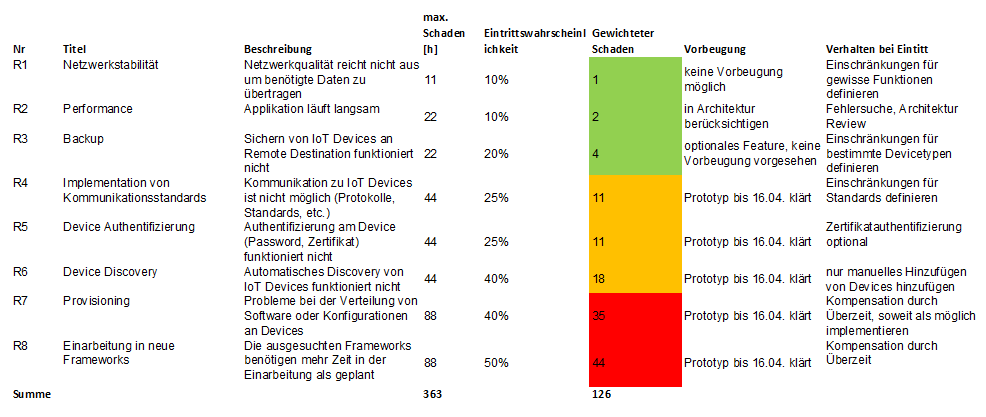
\includegraphics[scale=0.9]{../01_Projektplanung/images/risikoanalyse.png}
\caption{Risikoanalyse}
\end{figure}
\end{landscape}
\subsection{Umgang mit Risiken}
Die im Dokument aufgeführten Risiken sind in der Zeitplanung nicht speziell vorgesehen. Falls beim Eintreten eines geplanten Risikos ein erhöhter Zeitbedarf entsteht, so muss dies mit hoher Wahrscheinlichkeit mit Mehrarbeit der Teammitglieder kompensiert werden. Falls die nötige Mehrarbeit ausserhalb der Möglichkeiten liegt, so muss in Absprache aller Teammitglieder mit dem Betreuer nach einer anderer Lösung (z.B. Einschränkung von Programmfeatures, etc.) gesucht werden.